\subsection{Enunciado}
Se desea dividir un conjunto de $n$ personas para formar dos equipos que competirán entre sí.
Cada persona tiene un cierto nivel de competición, que viene representado por una puntuación
(un valor numérico entero). Con el objeto de que los dos equipos tengan un nivel similar,
se pretende construir los equipos de forma que la suma de las puntuaciones de sus miembros
sea lo m ás similar posible. Diseña e implementa un algoritmo vuelta atrás para resolver este
problema. Realizar un estudio empírico de la eficiencia de los algoritmos.

\subsection{Explicación}
Para simplificar el problema y darle mayor flexibilidad identificamos a cada jugador única y exlusivamente por su puntuación, aunque pueda haber dos jugadores con la misma puntuación. 
Esto permite que si hay dos jugadores con nivel de competición $x$ e $y$ con $x=y$ y cada uno está en un equipo podrían intercambiar sus posiciones sin descompensar los equipos.

Tenemos $n$ jugadores con puntuación respectiva $x_i\ \forall i\in I=[1, 1000]\cap \mathbb{N}$. 
Si inicialmente tuviésemos los niveles de los jugadores en otro rango $J=[a, b]\ a,b\in\mathbb{N}: a<b$ podemos dejarlo así, ya que el rango de los niveles no afecta al problema, salvo que apliquemos una transformación que reduzca el rango, ya que podríamos perder información al aproximar los números a enteros.

En cualquier caso la transformación al dominio del problema del intervalo $J$ es: $\forall j\in J$ aplicamos una función $F:[a,b] \rightarrow [1,1000]\cap\mathbb{N}$, teniendo en cuenta que $E(x)$ es la función parte entera:
\[F(x) = \left\{
	\begin{matrix}
		E\left( \frac{x-a}{b-a}\cdot 1000 \right)+1  & 
		\mbox{si } \left( \frac{x-a}{b-a}\cdot 1000 \right) < 
					E\left( \frac{x-a}{b-a}\cdot 1000 \right) + 1/2

	 \\	E\left( \frac{x-a}{b-a}\cdot 1000 \right)    & 
	 	\mbox{en otro caso}
	\end{matrix}
	\right.
\]

\subsection{Eficiencia}
En cuanto a la eficiencia de este algoritmo, podemos representar los $n$ jugadores como un vector de booleanos, donde si un jugador toma el valor \textit{true} está en un equipo y si toma el valor \textit{false} está en otro. De esta forma observamos que podemos representar la división por equipos en un único vector.

Tomando el primer jugador, puede estar en un equipo o en otro, $2$ combinaciones. Cogemos el siguiente jugador, puede estar en uno u otro, independientemente de donde estuviese el anterior, $2^2$ combinaciones. El tercer jugador vuelve a tener $2$ opciones, independientes del resto, $2^3$ combinaciones. 

Al tratarse de un algoritmo de vuelta atrás (backtraking) tenemos que recorrer todas las opciones, por lo que el problema queda representado como un árbol binario donde cada nodo tiene dos opciones, estar en un equipo o en otro.

\begin{figure}[H]
    \centering
    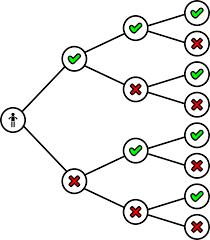
\includegraphics[scale=0.75]{./Imagenes/arbolbin.png}
    \caption{Distribución de equipos}
    \label{fig:arbolbin}
\end{figure}

De aquí deducimos la eficiencia del algoritmo con respecto al número total de jugadores $O(n)=2^n$.

Llegados a este punto nos podríamos plantear si podemos mejorar el algoritmo, curiosamente una forma de mejorarlo será ponerle una restricción, ya que nos ahorrará cálculos. 
La restricción nombrada será forzar que el número de jugadores en los dos equipos sea parecido, la diferencia de jugadores entre ambos equipos no será mayor de $1$. 
Esto hace que si hay un número de jugadores par ambos equipos siempre tengan el mismo número de jugadores. 
Ahorramos comprobaciones, pero el algoritmo sigue teniendo eficiencia $O(n)=2^n$ ya que pasaremos por todas las opciones, pero cuando la combinación en la que estemos no cumpla esa restricción la ignoraremos, sin hacer los cálculos asociados. 
La ventaja de este planteamiento se verá más adelante.


\subsection{Comparando ambos algoritmos}
El rango de jugadores usado ha sido $I=[3,26]\cap\mathbb{N}$, vemos como el estudio empírico corrobora las anteriores deduciones. 
Hemos ajustado funciones $f(n)=a \cdot 2^n\ a\in\mathbb{R}	\ \forall n\in I$. Sus coeficientes $r^2$ son $1$ en ambos casos (hay pocos elementos debido a la eficiencia) y el término $a$ está especificado en las gráficas, aunque también se encuentra en el archivo \textit{Equipos/Datos/ajustes.txt}.

\subsubsection{Tiempos}
\begin{figure}[H]
    \centering
    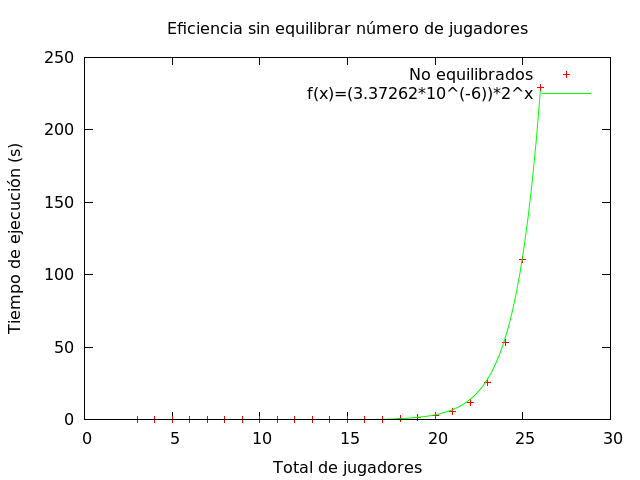
\includegraphics[scale=0.5]{../Equipos/Graficas/sinEquilibrar.png}
    \caption{Distribución de equipos sin equilibrar}
    \label{fig:Sin equilibrar}
\end{figure}

\vspace{0.5cm}

\begin{figure}[H]
    \centering
    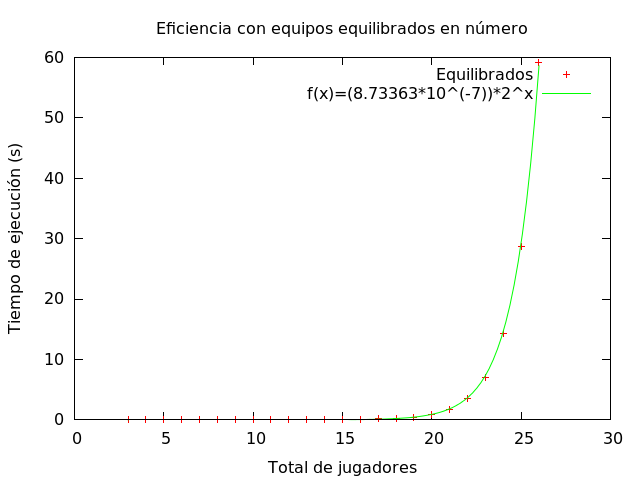
\includegraphics[scale=0.5]{../Equipos/Graficas/equilibrar.png}
    \caption{Distribución de equipos equilibrados en número}
    \label{fig:Equilibrado}
\end{figure}

Comparando ambos tiempos:

\begin{figure}[H]
    \centering
    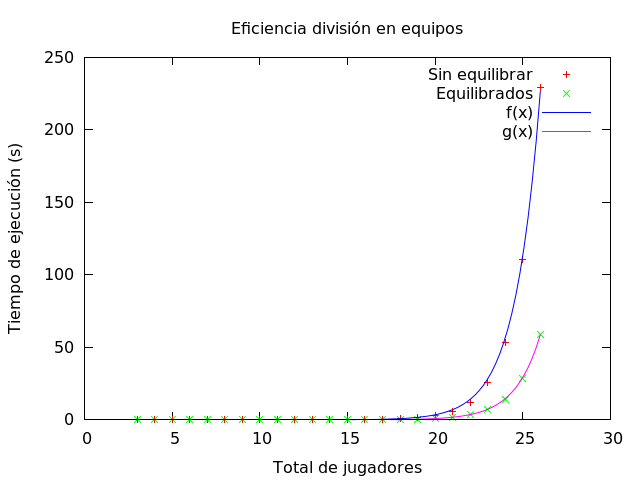
\includegraphics[scale=0.5]{../Equipos/Graficas/tiempos.png}
    \caption{Comparativa de tiempo}
    \label{fig:divisionTiempos}
\end{figure}

\subsubsection{Diferencia de nivel}
Recordemos que un jugador tiene un nivel entre $1$ y $1000$, es lógico pensar que con pocos jugadores el margen de optimización del algoritmo es menor debido al gran peso que toma la aleatoriedad con la que se determinan los niveles.
\begin{figure}[H]
    \centering
    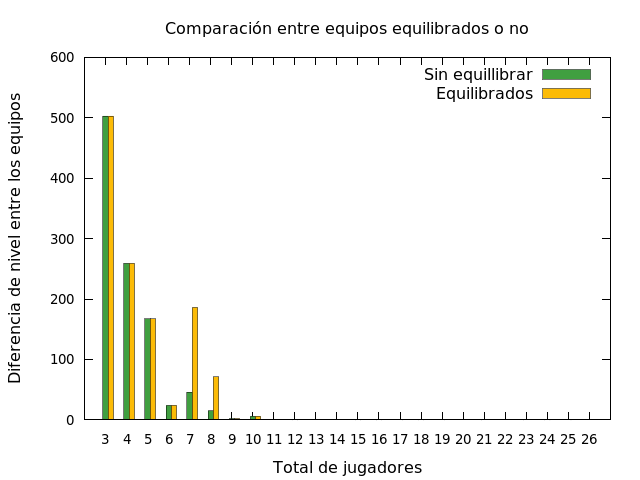
\includegraphics[scale=0.5]{../Equipos/Graficas/comparativa.png}
    \caption{Diferencia de nivel en los equipos}
    \label{fig:nivel}
\end{figure}

\subsubsection{Diferencia de jugadores}
El primer algoritmo tiende a desajustar el número de jugadores, llegando a tener los equipos una diferencia de $4$ jugadores cuando siendo $24$ en total.

\begin{figure}[H]
    \centering
    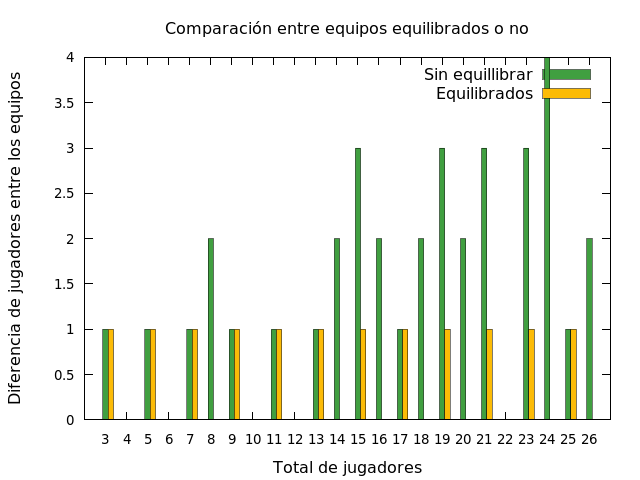
\includegraphics[scale=0.5]{../Equipos/Graficas/separacion.png}
    \caption{Diferencia en número de jugadores}
    \label{fig:separacion}
\end{figure}

\subsection{Conclusión}
Al ver esta eficiencia exponencial, si tenemos valores mayores de $30$ nos plantearemos algoritmos más rápidos. 
Para ejecuciones con un número pequeño de elementos los algoritmos planteados nos sirven, pero si aumentamos el número esa fuerza bruta no es tan buena idea.

Una forma de reducir las constantes ocultas es intentar ahorrarnos comprobaciones. 
Podríamos podar del árbol de soluciones, lo que denominaremos ``Branch and Bound".
También podríamos conformarnos con que la diferencia de nivel fuese menor que un $n\in\mathbb{N}$, de forma que no seguiríamos recorriendo el árbol una vez encontrada una solución satistactoria. 
Otra opción para disminuir el tiempo es paralelizar el problema, podemos hacer que cada procesador compruebe una rama diviendo el tiempo total.

Como hemos comprobado, el segundo algoritmo iguala al primero en eficacia, pero lo supera en eficiencia. 
Esto nos hace pensar que puede no ser necesario siempre recorrer el árbol de soluciones para asegurarnos la optimalidad.
